% Options for packages loaded elsewhere
\PassOptionsToPackage{unicode}{hyperref}
\PassOptionsToPackage{hyphens}{url}
%
\documentclass[
]{article}
\usepackage{amsmath,amssymb}
\usepackage{iftex}
\ifPDFTeX
  \usepackage[T1]{fontenc}
  \usepackage[utf8]{inputenc}
  \usepackage{textcomp} % provide euro and other symbols
\else % if luatex or xetex
  \usepackage{unicode-math} % this also loads fontspec
  \defaultfontfeatures{Scale=MatchLowercase}
  \defaultfontfeatures[\rmfamily]{Ligatures=TeX,Scale=1}
\fi
\usepackage{lmodern}
\ifPDFTeX\else
  % xetex/luatex font selection
\fi
% Use upquote if available, for straight quotes in verbatim environments
\IfFileExists{upquote.sty}{\usepackage{upquote}}{}
\IfFileExists{microtype.sty}{% use microtype if available
  \usepackage[]{microtype}
  \UseMicrotypeSet[protrusion]{basicmath} % disable protrusion for tt fonts
}{}
\makeatletter
\@ifundefined{KOMAClassName}{% if non-KOMA class
  \IfFileExists{parskip.sty}{%
    \usepackage{parskip}
  }{% else
    \setlength{\parindent}{0pt}
    \setlength{\parskip}{6pt plus 2pt minus 1pt}}
}{% if KOMA class
  \KOMAoptions{parskip=half}}
\makeatother
\usepackage{xcolor}
\usepackage[margin=1in]{geometry}
\usepackage{color}
\usepackage{fancyvrb}
\newcommand{\VerbBar}{|}
\newcommand{\VERB}{\Verb[commandchars=\\\{\}]}
\DefineVerbatimEnvironment{Highlighting}{Verbatim}{commandchars=\\\{\}}
% Add ',fontsize=\small' for more characters per line
\usepackage{framed}
\definecolor{shadecolor}{RGB}{248,248,248}
\newenvironment{Shaded}{\begin{snugshade}}{\end{snugshade}}
\newcommand{\AlertTok}[1]{\textcolor[rgb]{0.94,0.16,0.16}{#1}}
\newcommand{\AnnotationTok}[1]{\textcolor[rgb]{0.56,0.35,0.01}{\textbf{\textit{#1}}}}
\newcommand{\AttributeTok}[1]{\textcolor[rgb]{0.13,0.29,0.53}{#1}}
\newcommand{\BaseNTok}[1]{\textcolor[rgb]{0.00,0.00,0.81}{#1}}
\newcommand{\BuiltInTok}[1]{#1}
\newcommand{\CharTok}[1]{\textcolor[rgb]{0.31,0.60,0.02}{#1}}
\newcommand{\CommentTok}[1]{\textcolor[rgb]{0.56,0.35,0.01}{\textit{#1}}}
\newcommand{\CommentVarTok}[1]{\textcolor[rgb]{0.56,0.35,0.01}{\textbf{\textit{#1}}}}
\newcommand{\ConstantTok}[1]{\textcolor[rgb]{0.56,0.35,0.01}{#1}}
\newcommand{\ControlFlowTok}[1]{\textcolor[rgb]{0.13,0.29,0.53}{\textbf{#1}}}
\newcommand{\DataTypeTok}[1]{\textcolor[rgb]{0.13,0.29,0.53}{#1}}
\newcommand{\DecValTok}[1]{\textcolor[rgb]{0.00,0.00,0.81}{#1}}
\newcommand{\DocumentationTok}[1]{\textcolor[rgb]{0.56,0.35,0.01}{\textbf{\textit{#1}}}}
\newcommand{\ErrorTok}[1]{\textcolor[rgb]{0.64,0.00,0.00}{\textbf{#1}}}
\newcommand{\ExtensionTok}[1]{#1}
\newcommand{\FloatTok}[1]{\textcolor[rgb]{0.00,0.00,0.81}{#1}}
\newcommand{\FunctionTok}[1]{\textcolor[rgb]{0.13,0.29,0.53}{\textbf{#1}}}
\newcommand{\ImportTok}[1]{#1}
\newcommand{\InformationTok}[1]{\textcolor[rgb]{0.56,0.35,0.01}{\textbf{\textit{#1}}}}
\newcommand{\KeywordTok}[1]{\textcolor[rgb]{0.13,0.29,0.53}{\textbf{#1}}}
\newcommand{\NormalTok}[1]{#1}
\newcommand{\OperatorTok}[1]{\textcolor[rgb]{0.81,0.36,0.00}{\textbf{#1}}}
\newcommand{\OtherTok}[1]{\textcolor[rgb]{0.56,0.35,0.01}{#1}}
\newcommand{\PreprocessorTok}[1]{\textcolor[rgb]{0.56,0.35,0.01}{\textit{#1}}}
\newcommand{\RegionMarkerTok}[1]{#1}
\newcommand{\SpecialCharTok}[1]{\textcolor[rgb]{0.81,0.36,0.00}{\textbf{#1}}}
\newcommand{\SpecialStringTok}[1]{\textcolor[rgb]{0.31,0.60,0.02}{#1}}
\newcommand{\StringTok}[1]{\textcolor[rgb]{0.31,0.60,0.02}{#1}}
\newcommand{\VariableTok}[1]{\textcolor[rgb]{0.00,0.00,0.00}{#1}}
\newcommand{\VerbatimStringTok}[1]{\textcolor[rgb]{0.31,0.60,0.02}{#1}}
\newcommand{\WarningTok}[1]{\textcolor[rgb]{0.56,0.35,0.01}{\textbf{\textit{#1}}}}
\usepackage{longtable,booktabs,array}
\usepackage{calc} % for calculating minipage widths
% Correct order of tables after \paragraph or \subparagraph
\usepackage{etoolbox}
\makeatletter
\patchcmd\longtable{\par}{\if@noskipsec\mbox{}\fi\par}{}{}
\makeatother
% Allow footnotes in longtable head/foot
\IfFileExists{footnotehyper.sty}{\usepackage{footnotehyper}}{\usepackage{footnote}}
\makesavenoteenv{longtable}
\usepackage{graphicx}
\makeatletter
\def\maxwidth{\ifdim\Gin@nat@width>\linewidth\linewidth\else\Gin@nat@width\fi}
\def\maxheight{\ifdim\Gin@nat@height>\textheight\textheight\else\Gin@nat@height\fi}
\makeatother
% Scale images if necessary, so that they will not overflow the page
% margins by default, and it is still possible to overwrite the defaults
% using explicit options in \includegraphics[width, height, ...]{}
\setkeys{Gin}{width=\maxwidth,height=\maxheight,keepaspectratio}
% Set default figure placement to htbp
\makeatletter
\def\fps@figure{htbp}
\makeatother
\setlength{\emergencystretch}{3em} % prevent overfull lines
\providecommand{\tightlist}{%
  \setlength{\itemsep}{0pt}\setlength{\parskip}{0pt}}
\setcounter{secnumdepth}{-\maxdimen} % remove section numbering
\ifLuaTeX
  \usepackage{selnolig}  % disable illegal ligatures
\fi
\usepackage{bookmark}
\IfFileExists{xurl.sty}{\usepackage{xurl}}{} % add URL line breaks if available
\urlstyle{same}
\hypersetup{
  pdftitle={Rmarkdown\_16S\_Ananlysis\_mibibio},
  pdfauthor={Simon Vandersanden},
  hidelinks,
  pdfcreator={LaTeX via pandoc}}

\title{Rmarkdown\_16S\_Ananlysis\_mibibio}
\author{Simon Vandersanden}
\date{2026-03-05}

\begin{document}
\maketitle

Loading in the necessary libraries for basic handeling

\begin{Shaded}
\begin{Highlighting}[]
\FunctionTok{library}\NormalTok{(phyloseq)}
\FunctionTok{library}\NormalTok{(dplyr)}
\end{Highlighting}
\end{Shaded}

\begin{verbatim}
## 
## Attaching package: 'dplyr'
\end{verbatim}

\begin{verbatim}
## The following objects are masked from 'package:stats':
## 
##     filter, lag
\end{verbatim}

\begin{verbatim}
## The following objects are masked from 'package:base':
## 
##     intersect, setdiff, setequal, union
\end{verbatim}

\begin{Shaded}
\begin{Highlighting}[]
\FunctionTok{library}\NormalTok{(picante)    }\CommentTok{\# For Phylogenetic Diversity}
\end{Highlighting}
\end{Shaded}

\begin{verbatim}
## Loading required package: ape
\end{verbatim}

\begin{verbatim}
## 
## Attaching package: 'ape'
\end{verbatim}

\begin{verbatim}
## The following object is masked from 'package:dplyr':
## 
##     where
\end{verbatim}

\begin{verbatim}
## Loading required package: vegan
\end{verbatim}

\begin{verbatim}
## Loading required package: permute
\end{verbatim}

\begin{verbatim}
## Loading required package: lattice
\end{verbatim}

\begin{verbatim}
## This is vegan 2.6-8
\end{verbatim}

\begin{verbatim}
## Loading required package: nlme
\end{verbatim}

\begin{verbatim}
## 
## Attaching package: 'nlme'
\end{verbatim}

\begin{verbatim}
## The following object is masked from 'package:dplyr':
## 
##     collapse
\end{verbatim}

\begin{Shaded}
\begin{Highlighting}[]
\FunctionTok{library}\NormalTok{(microbiome) }\CommentTok{\# For Dominance metrics}
\end{Highlighting}
\end{Shaded}

\begin{verbatim}
## Loading required package: ggplot2
\end{verbatim}

\begin{verbatim}
## 
## microbiome R package (microbiome.github.com)
##     
## 
## 
##  Copyright (C) 2011-2022 Leo Lahti, 
##     Sudarshan Shetty et al. <microbiome.github.io>
\end{verbatim}

\begin{verbatim}
## 
## Attaching package: 'microbiome'
\end{verbatim}

\begin{verbatim}
## The following object is masked from 'package:ggplot2':
## 
##     alpha
\end{verbatim}

\begin{verbatim}
## The following object is masked from 'package:vegan':
## 
##     diversity
\end{verbatim}

\begin{verbatim}
## The following object is masked from 'package:base':
## 
##     transform
\end{verbatim}

\begin{Shaded}
\begin{Highlighting}[]
\FunctionTok{library}\NormalTok{(vegan)      }\CommentTok{\# For Rarefaction curves}
\FunctionTok{library}\NormalTok{(zCompositions)}
\end{Highlighting}
\end{Shaded}

\begin{verbatim}
## Loading required package: MASS
\end{verbatim}

\begin{verbatim}
## 
## Attaching package: 'MASS'
\end{verbatim}

\begin{verbatim}
## The following object is masked from 'package:dplyr':
## 
##     select
\end{verbatim}

\begin{verbatim}
## Loading required package: truncnorm
\end{verbatim}

\begin{verbatim}
## Loading required package: survival
\end{verbatim}

\begin{Shaded}
\begin{Highlighting}[]
\FunctionTok{library}\NormalTok{(ggplot2)}
\FunctionTok{library}\NormalTok{(ggrepel)}
\FunctionTok{library}\NormalTok{(MicrobiomeStat)}
\FunctionTok{library}\NormalTok{(scales)}
\end{Highlighting}
\end{Shaded}

\begin{verbatim}
## 
## Attaching package: 'scales'
\end{verbatim}

\begin{verbatim}
## The following object is masked from 'package:microbiome':
## 
##     alpha
\end{verbatim}

\begin{Shaded}
\begin{Highlighting}[]
\FunctionTok{library}\NormalTok{(paletteer)}
\end{Highlighting}
\end{Shaded}

\subsection{1:Inspecting the different parts of the phyloseq
object}\label{inspecting-the-different-parts-of-the-phyloseq-object}

\begin{Shaded}
\begin{Highlighting}[]
\CommentTok{\#Load in the phyloseq object}
\NormalTok{mibi\_phylo\_object }\OtherTok{\textless{}{-}} \FunctionTok{readRDS}\NormalTok{(}\StringTok{"data/ps\_IdTax\_noncontam\_NoMitChlo\_Tree.rds"}\NormalTok{) }
\CommentTok{\# To see the OTU table}
\NormalTok{mibi\_otu\_table}\OtherTok{\textless{}{-}} \FunctionTok{as}\NormalTok{(}\FunctionTok{otu\_table}\NormalTok{(mibi\_phylo\_object), }\StringTok{"matrix"}\NormalTok{)}
\CommentTok{\#head(mibi\_otu\_table[,1:5])}
\CommentTok{\# To see the Taxonomy}
\NormalTok{mibi\_tax\_table }\OtherTok{\textless{}{-}} \FunctionTok{as}\NormalTok{(}\FunctionTok{tax\_table}\NormalTok{(mibi\_phylo\_object), }\StringTok{"matrix"}\NormalTok{)}
\CommentTok{\#head(mibi\_tax\_table)}
\CommentTok{\# To see the Metadata}
\NormalTok{mibi\_meta\_table }\OtherTok{\textless{}{-}} \FunctionTok{as}\NormalTok{(}\FunctionTok{sample\_data}\NormalTok{(mibi\_phylo\_object), }\StringTok{"data.frame"}\NormalTok{)}
\CommentTok{\#head(mibi\_tax\_table)}

\CommentTok{\# You can also swap the metadata table, in case you want to make adjustments to the grouping of the samples or add some new metadata the the specific samples}
\NormalTok{mibi\_meta\_table\_new }\OtherTok{\textless{}{-}} \FunctionTok{read.table}\NormalTok{(}\StringTok{"data/META\_Griftpark\_Soilcore\_Measurements.txt"}\NormalTok{, }\AttributeTok{header =}\NormalTok{ T, }\AttributeTok{sep =} \StringTok{"}\SpecialCharTok{\textbackslash{}t}\StringTok{"}\NormalTok{, }\AttributeTok{row.names =} \DecValTok{1}\NormalTok{, }\AttributeTok{stringsAsFactors =} \ConstantTok{FALSE}\NormalTok{, }\AttributeTok{dec =} \StringTok{\textquotesingle{},\textquotesingle{}}\NormalTok{)}
\CommentTok{\#Make sure the rownames of the loaded in metadata match the sample names in the phyloseq object}
\FunctionTok{stopifnot}\NormalTok{(}\FunctionTok{all}\NormalTok{(}\FunctionTok{sample\_names}\NormalTok{(mibi\_phylo\_object) }\SpecialCharTok{\%in\%} \FunctionTok{rownames}\NormalTok{(mibi\_meta\_table\_new)))}

\FunctionTok{sample\_data}\NormalTok{(mibi\_phylo\_object) }\OtherTok{\textless{}{-}}\NormalTok{ mibi\_meta\_table\_new}

\CommentTok{\#After this step you have the otu count table information, the taxonomy table and the correct or an updated version of the metadata}
\end{Highlighting}
\end{Shaded}

\subsection{2.1:Data Pre-processing: Filtering out all non-samples and
checking rarefaction
curves}\label{data-pre-processing-filtering-out-all-non-samples-and-checking-rarefaction-curves}

\begin{Shaded}
\begin{Highlighting}[]
\CommentTok{\#Normally some pre filtering has been done on the reads before they were put into the phyloseq object: the sequencing depth threshhold, the decontamination, and some taxonomic filtering of certain undesired taxa such as Eukaryota, Mitochondria and Chloroplast sequences.}

\CommentTok{\# It is possible that that some blancs and mock samples are still present in the samples, these should be filtered out because we will only filter using all the \textquotesingle{}real samples\textquotesingle{}}
\CommentTok{\#filter out these blanc samples:}
\NormalTok{samples\_to\_remove }\OtherTok{\textless{}{-}} \FunctionTok{c}\NormalTok{(}\StringTok{"Blank"}\NormalTok{, }\StringTok{"MockB"}\NormalTok{, }\StringTok{"nosample1"}\NormalTok{, }\StringTok{"nosample2"}\NormalTok{, }\StringTok{"nosample3"}\NormalTok{, }\StringTok{"nosample4"}\NormalTok{)}
\NormalTok{mibi\_phylo\_object }\OtherTok{\textless{}{-}} \FunctionTok{prune\_samples}\NormalTok{(}
  \SpecialCharTok{!}\NormalTok{(}\FunctionTok{sample\_names}\NormalTok{(mibi\_phylo\_object) }\SpecialCharTok{\%in\%}\NormalTok{ samples\_to\_remove),}
\NormalTok{  mibi\_phylo\_object}
\NormalTok{)}
\CommentTok{\# Check the rarefaction curves:}
\CommentTok{\#Requires: mibi\_phylo\_object}
\FunctionTok{source}\NormalTok{(}\StringTok{"scripts/02\_rarefaction\_curves.R"}\NormalTok{)}
\end{Highlighting}
\end{Shaded}

\begin{verbatim}
## Calculating rarefaction curves... this may take a moment.
\end{verbatim}

\begin{verbatim}
## Warning in vegan::rarecurve(otu_rare, step = 100, cex = 0.5, label = FALSE, :
## most observed count data have counts 1, but smallest count is 2
\end{verbatim}

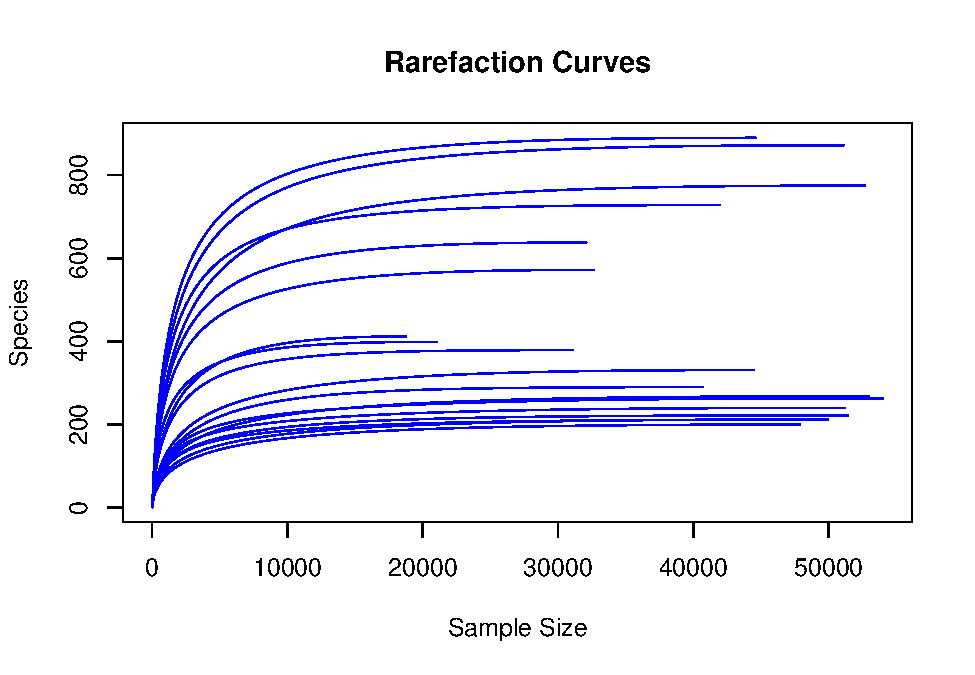
\includegraphics{Pipeline_Overview_files/figure-latex/unnamed-chunk-3-1.pdf}

\subsection{2.1:Data Pre-processing: Filtering out based on prevalence
and
abundance}\label{data-pre-processing-filtering-out-based-on-prevalence-and-abundance}

\begin{Shaded}
\begin{Highlighting}[]
\CommentTok{\# {-}{-}{-} Filtering parameters:USER INPUT SECTION {-}{-}{-}}
\CommentTok{\# Thresholds}
\NormalTok{prev\_filter\_threshold }\OtherTok{=} \DecValTok{3}   \CommentTok{\# Present in at least X samples}
\NormalTok{abund\_filter\_threshold }\OtherTok{=} \DecValTok{5} \CommentTok{\# At least X reads }

\CommentTok{\# Logic Switches (1 = On, 0 = Off)}
  \CommentTok{\# Here you can specify which filtering must be done,}
  \CommentTok{\# Only based on prevalence, or abudance. Then fill in a 0 accordingly}
  \CommentTok{\# Most of the time it is a combination of both prevalence and abundance, for example, at least \textgreater{}10 reads in 5 samples.}
\NormalTok{prev\_filter }\OtherTok{=} \DecValTok{1} 
\NormalTok{abund\_filter }\OtherTok{=} \DecValTok{1}
\CommentTok{\# {-}{-}{-}{-}{-}{-}{-}{-}{-}{-}{-}{-}{-}{-}{-}{-}{-}{-}{-}{-}{-}{-}{-}{-}{-}{-}}
\CommentTok{\# Run the background script}
\CommentTok{\# Requires: mibi\_phylo\_object, prev\_filter\_threshold, abund\_filter\_threshold...}
\FunctionTok{source}\NormalTok{(}\StringTok{"scripts/02\_filtering\_prevalence\_abundance.R"}\NormalTok{)}
\end{Highlighting}
\end{Shaded}

\begin{verbatim}
## --- Filtering Summary ---
\end{verbatim}

\begin{verbatim}
## Criteria: Combined (min 5 reads in 3 samples)
\end{verbatim}

\begin{verbatim}
## Taxa before: 4427
\end{verbatim}

\begin{verbatim}
## Taxa after:  964
\end{verbatim}

\begin{verbatim}
## Percent kept: 21.78%
\end{verbatim}

\begin{verbatim}
## -------------------------
\end{verbatim}

\begin{Shaded}
\begin{Highlighting}[]
\CommentTok{\#The script starts with taking the mibi\_phylo\_object and makes the: }
\CommentTok{\#The resulting object \textquotesingle{}mibi\_phylo\_object\_filt\textquotesingle{} is now ready }
\end{Highlighting}
\end{Shaded}

\subsection{2.1:Data Pre-processing: Filtering based on variance
OPTIONAL, !!!This is not working yet!!!Also this should not be used for
alpha or beta diversity, However it might be usefull before differential
abundance
analysis}\label{data-pre-processing-filtering-based-on-variance-optional-this-is-not-working-yetalso-this-should-not-be-used-for-alpha-or-beta-diversity-however-it-might-be-usefull-before-differential-abundance-analysis}

\begin{Shaded}
\begin{Highlighting}[]
\CommentTok{\#Check the distribution of the varriances }
\NormalTok{otu }\OtherTok{\textless{}{-}} \FunctionTok{as.matrix}\NormalTok{(microbiome}\SpecialCharTok{::}\FunctionTok{abundances}\NormalTok{(mibi\_phylo\_object\_filt))}
\NormalTok{taxon\_variance }\OtherTok{\textless{}{-}} \FunctionTok{apply}\NormalTok{(otu, }\DecValTok{1}\NormalTok{, IQR)}
\NormalTok{taxon\_variance }\OtherTok{\textless{}{-}} \FunctionTok{apply}\NormalTok{(}\FunctionTok{as.matrix}\NormalTok{(microbiome}\SpecialCharTok{::}\FunctionTok{abundances}\NormalTok{(mibi\_phylo\_object\_filt)), }\DecValTok{1}\NormalTok{, IQR)}\SpecialCharTok{\textgreater{}} \FunctionTok{quantile}\NormalTok{(taxon\_variance, }\AttributeTok{probs =} \FunctionTok{seq}\NormalTok{(}\DecValTok{0}\NormalTok{, }\DecValTok{1}\NormalTok{, }\FloatTok{0.05}\NormalTok{))}
\end{Highlighting}
\end{Shaded}

\begin{verbatim}
## Warning in apply(as.matrix(microbiome::abundances(mibi_phylo_object_filt)), :
## longer object length is not a multiple of shorter object length
\end{verbatim}

\begin{Shaded}
\begin{Highlighting}[]
\CommentTok{\#This will remove a lot of taxa, since there will be many taxa with 0 variance because they only occur in one sample.}
\CommentTok{\# {-}{-}{-} Filtering parameters: USER INPUT SECTION {-}{-}{-}}
\CommentTok{\# Variance Cutoff (e.g., 0.1 removes the bottom 10\% least variable taxa)}
\NormalTok{variance\_cutoff }\OtherTok{=} \FloatTok{0.00}

\CommentTok{\# Logic Switch (1 = On, 0 = Off)}
\NormalTok{variance\_filter\_switch }\OtherTok{=} \DecValTok{1} 
\CommentTok{\# {-}{-}{-}{-}{-}{-}{-}{-}{-}{-}{-}{-}{-}{-}{-}{-}{-}{-}{-}{-}{-}{-}{-}{-}{-}{-}}
\CommentTok{\# Run the background script}
\FunctionTok{source}\NormalTok{(}\StringTok{"scripts/02\_filtering\_variance.R"}\NormalTok{)}
\end{Highlighting}
\end{Shaded}

\begin{verbatim}
## Filtering applied: Low variance (Interquartile Range). (Threshold was 0; dropped all absolute zero-variance taxa)
\end{verbatim}

\begin{verbatim}
## Variance Filter: Excluded the bottom 0% taxa. Removed: 626 ASVs.
## Final taxa count: 338
\end{verbatim}

\begin{Shaded}
\begin{Highlighting}[]
\CommentTok{\#This script starts with mibi\_phylo\_object\_filt and updates it with this filtering }
\CommentTok{\# The resulting object \textquotesingle{}mibi\_phylo\_object\_filt\textquotesingle{} is now updated}
\end{Highlighting}
\end{Shaded}

\subsection{2.1:Data Pre-processing: Sample removal or subset
selection}\label{data-pre-processing-sample-removal-or-subset-selection}

\begin{Shaded}
\begin{Highlighting}[]
\CommentTok{\#Define the target group you want to subset}
\NormalTok{target\_group }\OtherTok{=} \StringTok{\textquotesingle{}SC6\textquotesingle{}}
\CommentTok{\# 1. Subset the samples}
\NormalTok{mibi\_phylo\_object\_subset }\OtherTok{\textless{}{-}} \FunctionTok{subset\_samples}\NormalTok{(mibi\_phylo\_object\_filt, SC\_Number }\SpecialCharTok{==}\NormalTok{ target\_group)}

\CommentTok{\# 2. Corrected Pruning: Sum the counts within the NEW subset}
\CommentTok{\# This ensures that if an ASV only existed in \textquotesingle{}SC1\textquotesingle{}, it is removed from the \textquotesingle{}SC2\textquotesingle{} object.}
\NormalTok{mibi\_phylo\_object\_subset }\OtherTok{\textless{}{-}} \FunctionTok{prune\_taxa}\NormalTok{(}\FunctionTok{taxa\_sums}\NormalTok{(mibi\_phylo\_object\_subset) }\SpecialCharTok{\textgreater{}} \DecValTok{0}\NormalTok{, mibi\_phylo\_object\_subset)}

\CommentTok{\# 3. Reporting (Partners love to see how much was lost)}
\FunctionTok{message}\NormalTok{(}\FunctionTok{paste}\NormalTok{(}\StringTok{"Subset selected:"}\NormalTok{, target\_group))}
\end{Highlighting}
\end{Shaded}

\begin{verbatim}
## Subset selected: SC6
\end{verbatim}

\begin{Shaded}
\begin{Highlighting}[]
\FunctionTok{message}\NormalTok{(}\FunctionTok{paste}\NormalTok{(}\StringTok{"Samples remaining:"}\NormalTok{, }\FunctionTok{nsamples}\NormalTok{(mibi\_phylo\_object\_subset)))}
\end{Highlighting}
\end{Shaded}

\begin{verbatim}
## Samples remaining: 3
\end{verbatim}

\begin{Shaded}
\begin{Highlighting}[]
\FunctionTok{message}\NormalTok{(}\FunctionTok{paste}\NormalTok{(}\StringTok{"Taxa remaining after pruning zeros:"}\NormalTok{, }\FunctionTok{ntaxa}\NormalTok{(mibi\_phylo\_object\_subset)))}
\end{Highlighting}
\end{Shaded}

\begin{verbatim}
## Taxa remaining after pruning zeros: 131
\end{verbatim}

\subsection{2.2 Object Finalization, selecting the object for the data
analysis and
normalisation}\label{object-finalization-selecting-the-object-for-the-data-analysis-and-normalisation}

\begin{Shaded}
\begin{Highlighting}[]
\DocumentationTok{\#\# 2.3 Object Finalization}
\CommentTok{\# Define which object flows into the analysis scripts}
\CommentTok{\# Options: mibi\_phylo\_object\_filt (full) or mibi\_phylo\_object\_subset (subset)}
\NormalTok{ps\_work }\OtherTok{\textless{}{-}}\NormalTok{ mibi\_phylo\_object\_filt}
\CommentTok{\#str(ps\_work)}
\end{Highlighting}
\end{Shaded}

2.2:Data Pre-processing: Normalisation \#\# 3.0 Normalization \& The
``Zero Problem''

Microbiome data is \textbf{compositional}. Because total read counts are
an artifact of sequencer depth, they represent ``parts of a whole''
rather than absolute concentrations. If one taxon blooms, others appear
to decrease simply because they occupy a smaller percentage of the total
pool.

\subsubsection{3.1 Handling Sparsity (Zero
Imputation)}\label{handling-sparsity-zero-imputation}

Log-ratio transformations (like CLR) cannot handle zeros because
\(\log(0)\) is undefined. We address this using two distinct approaches
before transformation:

\begin{itemize}
\tightlist
\item
  \textbf{Simple Pseudo-count (+1):} Adds a constant shift of 1 to every
  cell. It is fast and robust, though it can slightly bias ratios in
  extremely sparse datasets.
\item
  \textbf{Bayesian-Multiplicative Replacement (BMR):} Uses the
  \texttt{zCompositions} package to impute zeros based on a Dirichlet
  prior. This is more mathematically rigorous as it preserves the ratio
  structure of the data.

  \begin{itemize}
  \tightlist
  \item
    \textbf{Note:} BMR requires careful handling of ``singletons.'' We
    have adjusted the \texttt{z.delete} and \texttt{z.warning}
    thresholds to ensure samples with limited diversity are not dropped
    during the imputation process.
  \end{itemize}
\item
  \textbf{Matrix Completion:} \emph{Planned for future implementation.}
\end{itemize}

\begin{center}\rule{0.5\linewidth}{0.5pt}\end{center}

\subsubsection{3.2 Executed
Transformations}\label{executed-transformations}

The following background script processes the chosen \texttt{ps\_work}
object and generates the normalized data structures, using different
techniques.

\begin{Shaded}
\begin{Highlighting}[]
\CommentTok{\# Requires: ps\_work (defined in the data pre{-}processing section)}
\FunctionTok{source}\NormalTok{(}\StringTok{"scripts/03\_normalisation.R"}\NormalTok{)}
\end{Highlighting}
\end{Shaded}

\begin{verbatim}
## Attempting BMR zero-imputation with microbiome-specific settings...
\end{verbatim}

\begin{verbatim}
## No. adjusted imputations:  3059
\end{verbatim}

\begin{verbatim}
## BMR successful: Imputed counts integrated.
\end{verbatim}

\begin{verbatim}
## --- Normalization Summary ---
\end{verbatim}

\begin{verbatim}
## 1. TSS: Relative abundance (0-100%) created.
\end{verbatim}

\begin{verbatim}
## 2. Pseudo-CLR: Fast +1 shift transformation created.
\end{verbatim}

\begin{verbatim}
## 3. BMR-CLR: Bayesian-imputed transformation created.
\end{verbatim}

\begin{verbatim}
## -----------------------------
\end{verbatim}

\begin{Shaded}
\begin{Highlighting}[]
\CommentTok{\#The following objects are created:}
\CommentTok{\#mibi\_tss}
\CommentTok{\#mibi\_pseudo\_clr}
\CommentTok{\#mibi\_bmr\_clr}
\end{Highlighting}
\end{Shaded}

\#\#\#The script generates three primary objects. Choosing the right one
depends on your specific analysis:

-mibi\_tss Total Sum Scaling Visualization: Relative Abundance (\%) used
for stacked bar plots.

-mibi\_pseudo\_clr Pseudo-CLR (+1) Statistics: Fast transformation for
PCoA and basic linear modeling.

-mibi\_bmr\_clr BMR-CLR (Bayesian) Advanced Stats: High-fidelity
modeling and differential abundance.

\subsection{Community visualisation:
barplots}\label{community-visualisation-barplots}

\#This chunk of code is designed to plot relative abundances of you
microbial community data, this takes the microbial community and you can
select at which level the plotting is done, the labeling is two levels
to ensure comprehensiveness, and detail (higher phylogenetic level and
lower for the detail). The main color is determined by the high level
taxonomy, variations of this main color are used in the lower levels.
Several choices can be made, a relative abundance threshold level, which
is a cutoff level for relative abundance, if a taxon does not meet this
threshold i.e.~all taxa with relative abundance belower this threshold
are put into `Others'

\begin{Shaded}
\begin{Highlighting}[]
\CommentTok{\# {-}{-}{-} SETUP, load in the script that is the code backbone of this part {-}{-}{-}}
\FunctionTok{source}\NormalTok{(}\StringTok{"scripts/08\_barchart\_visualisation.R"}\NormalTok{)}
\end{Highlighting}
\end{Shaded}

\begin{verbatim}
## -- Attaching core tidyverse packages ------------------------ tidyverse 2.0.0 --
## v forcats   1.0.0     v stringr   1.5.2
## v lubridate 1.9.4     v tibble    3.2.1
## v purrr     1.1.0     v tidyr     1.3.1
## v readr     2.1.5     
## -- Conflicts ------------------------------------------ tidyverse_conflicts() --
## x scales::alpha()     masks microbiome::alpha(), ggplot2::alpha()
## x readr::col_factor() masks scales::col_factor()
## x nlme::collapse()    masks dplyr::collapse()
## x purrr::discard()    masks scales::discard()
## x dplyr::filter()     masks stats::filter()
## x dplyr::lag()        masks stats::lag()
## x MASS::select()      masks dplyr::select()
## x ape::where()        masks dplyr::where()
## i Use the conflicted package (<http://conflicted.r-lib.org/>) to force all conflicts to become errors
\end{verbatim}

\begin{Shaded}
\begin{Highlighting}[]
\CommentTok{\# {-}{-}{-} 1. INPUT {-}{-}{-}}
\CommentTok{\# specify the plot specifics:}
\NormalTok{high\_level }\OtherTok{\textless{}{-}} \StringTok{"order"} \CommentTok{\# Specify the high taxonomic level}
\NormalTok{low\_level  }\OtherTok{\textless{}{-}} \StringTok{"family"} \CommentTok{\# Specify the lower taxonomic level}
\NormalTok{facet\_var  }\OtherTok{\textless{}{-}} \StringTok{"Sample"} \CommentTok{\# or "Grouping\_SC or Sample"}
\NormalTok{threshold  }\OtherTok{\textless{}{-}} \DecValTok{1} \CommentTok{\# Specify the relative abundance threshold from which the taxa are filtered}
\NormalTok{pal\_choice  }\OtherTok{\textless{}{-}} \StringTok{"pals::polychrome"} \CommentTok{\# Define the color pallet to use}
\CommentTok{\# {-}{-}{-} 2. CREATION OF THE OBJECT FOR PLOTTING {-}{-}{-}}
\CommentTok{\# Here the previously defined taxa are put into the function that prepares the data for plotting.}
\NormalTok{data\_for\_plot }\OtherTok{\textless{}{-}} \FunctionTok{prepare\_abundance\_data}\NormalTok{(}
  \AttributeTok{ps         =}\NormalTok{ ps\_work, }\CommentTok{\#Here you specify the phyloseq object which you want to plot from}
  \AttributeTok{high\_level =}\NormalTok{ high\_level,}
  \AttributeTok{low\_level  =}\NormalTok{ low\_level, }
  \AttributeTok{facet\_var  =}\NormalTok{ facet\_var, }
  \AttributeTok{threshold  =}\NormalTok{ threshold )}
\CommentTok{\# This prepared the colours, so custom colours are assigned to the created groups depending on the taxonomic specification.}
\NormalTok{my\_colors }\OtherTok{\textless{}{-}} \FunctionTok{get\_shaded\_palette}\NormalTok{(data\_for\_plot, pal\_choice)}

\CommentTok{\# {-}{-}{-} 3. DYNAMIC PLOTTING {-}{-}{-}}
\CommentTok{\# This is a complex plotting command that is constructed to take into acount the previously specified parameters, high and low taxonomic levels, relative abundance threshold cutoff, how to group the samples for plotting. So this information is also found on the finally generated plot}
\NormalTok{Relative\_Abundance\_Plot }\OtherTok{\textless{}{-}} \FunctionTok{ggplot}\NormalTok{(data\_for\_plot, }\FunctionTok{aes}\NormalTok{(}\AttributeTok{x =} \SpecialCharTok{!!}\FunctionTok{sym}\NormalTok{(facet\_var), }\AttributeTok{y =}\NormalTok{ Abundance, }\AttributeTok{fill =}\NormalTok{ Hierarchical\_Label)) }\SpecialCharTok{+}
  \FunctionTok{geom\_bar}\NormalTok{(}\AttributeTok{stat =} \StringTok{"identity"}\NormalTok{, }\AttributeTok{position =} \StringTok{"stack"}\NormalTok{, }\AttributeTok{color =} \StringTok{"black"}\NormalTok{, }\AttributeTok{size =} \FloatTok{0.05}\NormalTok{) }\SpecialCharTok{+}
  \FunctionTok{scale\_fill\_manual}\NormalTok{(}\AttributeTok{values =}\NormalTok{ my\_colors) }\SpecialCharTok{+}
  \FunctionTok{labs}\NormalTok{(    }\AttributeTok{title =} \FunctionTok{paste}\NormalTok{(}\StringTok{"Relative Abundance:"}\NormalTok{, }\FunctionTok{str\_to\_title}\NormalTok{(high\_level), }\StringTok{"{-}"}\NormalTok{, }\FunctionTok{str\_to\_title}\NormalTok{(low\_level)),}
    \AttributeTok{subtitle =} \FunctionTok{paste}\NormalTok{(}\StringTok{"Filtered at"}\NormalTok{, threshold, }\StringTok{"\% threshold | Grouped by"}\NormalTok{, facet\_var),}
    \AttributeTok{x =} \FunctionTok{str\_replace\_all}\NormalTok{(facet\_var, }\StringTok{"\_"}\NormalTok{, }\StringTok{" "}\NormalTok{),}
    \AttributeTok{y =} \StringTok{"Relative Abundance (\%)"}\NormalTok{,}
    \AttributeTok{fill =} \FunctionTok{paste}\NormalTok{(}\FunctionTok{str\_to\_title}\NormalTok{(high\_level), }\StringTok{"{-}"}\NormalTok{, }\FunctionTok{str\_to\_title}\NormalTok{(low\_level))}
\NormalTok{  ) }\SpecialCharTok{+}
  \FunctionTok{theme\_minimal}\NormalTok{(}\AttributeTok{base\_size =} \DecValTok{12}\NormalTok{) }\SpecialCharTok{+}
  \FunctionTok{theme}\NormalTok{(}
    \AttributeTok{axis.text.x =} \FunctionTok{element\_text}\NormalTok{(}\AttributeTok{angle =} \DecValTok{45}\NormalTok{, }\AttributeTok{vjust =} \DecValTok{1}\NormalTok{, }\AttributeTok{hjust =} \DecValTok{1}\NormalTok{),}
    \AttributeTok{legend.text =} \FunctionTok{element\_text}\NormalTok{(}\AttributeTok{size =} \DecValTok{9}\NormalTok{),}
    \AttributeTok{panel.grid.major.x =} \FunctionTok{element\_blank}\NormalTok{(),}
    \AttributeTok{plot.title =} \FunctionTok{element\_text}\NormalTok{(}\AttributeTok{face =} \StringTok{"bold"}\NormalTok{)}
\NormalTok{  ) }\SpecialCharTok{+}
  \FunctionTok{guides}\NormalTok{(}\AttributeTok{fill =} \FunctionTok{guide\_legend}\NormalTok{(}\AttributeTok{ncol =} \DecValTok{2}\NormalTok{))}
\end{Highlighting}
\end{Shaded}

\begin{verbatim}
## Warning: Using `size` aesthetic for lines was deprecated in ggplot2 3.4.0.
## i Please use `linewidth` instead.
## This warning is displayed once every 8 hours.
## Call `lifecycle::last_lifecycle_warnings()` to see where this warning was
## generated.
\end{verbatim}

\begin{Shaded}
\begin{Highlighting}[]
\CommentTok{\# Display the plot}
\NormalTok{Relative\_Abundance\_Plot}
\end{Highlighting}
\end{Shaded}

\includegraphics{Pipeline_Overview_files/figure-latex/unnamed-chunk-9-1.pdf}

\begin{Shaded}
\begin{Highlighting}[]
\CommentTok{\#This chunk of code is designed to plot relative abundances of you microbial community data. But here you can look within specific group and get the lower level taxonomic distribution so you can gain insights into specific important groups within you data.The labeling is two levels to ensure comprehensiveness, and detail (higher phylogenetic level and lower for the detail). The main color is determined by the high level taxonomy, variations of this main color are used in the lower levels. Several choices can be made, a relative abundance threshold level, which is a cutoff level for relative abundance, if a taxon does not meet this threshold i.e. all taxa with relative abundance belower this threshold are put into \textquotesingle{}Others\textquotesingle{} }

\CommentTok{\# {-}{-}{-} 1. DEFINE SPECIFICS {-}{-}{-}}
\CommentTok{\# These two inputs are specific for this script. Here you select which specific taxon you want to take a closer look at}
\NormalTok{target\_rank }\OtherTok{\textless{}{-}} \StringTok{"order"} \CommentTok{\# "family", "order", "class" "phylum"}
\NormalTok{target\_val  }\OtherTok{\textless{}{-}} \StringTok{"Burkholderiales\_2"} \CommentTok{\# select the specific group within the target rank e.g. Pseudomonadota for the phylum. Burkholderiales for order}

\CommentTok{\# From this specifically selected group there is the possibility to plot the lower taxonomic levels within it, similar logic to a normal relative abundance plot, but now the relative abundance within this selected taxonomic group is plotted.}

\NormalTok{high\_level  }\OtherTok{\textless{}{-}} \StringTok{"family"}
\NormalTok{low\_level   }\OtherTok{\textless{}{-}} \StringTok{"genus"}
\NormalTok{facet\_var   }\OtherTok{\textless{}{-}} \StringTok{"Sample"}
\NormalTok{threshold   }\OtherTok{\textless{}{-}} \FloatTok{0.5} 
\NormalTok{pal\_choice  }\OtherTok{\textless{}{-}} \StringTok{"pals::polychrome"}

\CommentTok{\# {-}{-}{-} 2. CREATION OF THE OBJECT FOR PLOTTING {-}{-}{-}}
\CommentTok{\# Calls the subsetting function from 08\_barchart\_specific\_group.R}
\FunctionTok{source}\NormalTok{(}\StringTok{"scripts/08\_barchart\_specific\_group.R"}\NormalTok{)}
\NormalTok{data\_subset }\OtherTok{\textless{}{-}} \FunctionTok{prepare\_specific\_abundance\_data}\NormalTok{(}
  \AttributeTok{ps         =}\NormalTok{ ps\_work,}
  \AttributeTok{rank\_name  =}\NormalTok{ target\_rank,}
  \AttributeTok{rank\_value =}\NormalTok{ target\_val,}
  \AttributeTok{high\_level =}\NormalTok{ high\_level,}
  \AttributeTok{low\_level  =}\NormalTok{ low\_level,}
  \AttributeTok{facet\_var  =}\NormalTok{ facet\_var,}
  \AttributeTok{threshold  =}\NormalTok{ threshold}
\NormalTok{)}

\CommentTok{\# This prepared the colors, so custom colors are assigned to the created groups depending on the taxonomic specification.}
\NormalTok{my\_colors\_sub }\OtherTok{\textless{}{-}} \FunctionTok{get\_shaded\_palette}\NormalTok{(data\_subset, pal\_choice)}\CommentTok{\# Uses the shared function from 08\_barchart\_visualisation.R}

\CommentTok{\# {-}{-}{-} 3. DYNAMIC PLOTTING {-}{-}{-}}
\CommentTok{\# This is a complex plotting command that is constructed to take into acount the previously specified parameters, high and low taxonomic levels, relative abundance threshold cutoff, how to group the samples for plotting. So this information is also found on the finally generated plot}
\NormalTok{p\_sub }\OtherTok{\textless{}{-}} \FunctionTok{ggplot}\NormalTok{(data\_subset, }\FunctionTok{aes}\NormalTok{(}\AttributeTok{x =} \SpecialCharTok{!!}\FunctionTok{sym}\NormalTok{(facet\_var), }\AttributeTok{y =}\NormalTok{ Abundance, }\AttributeTok{fill =}\NormalTok{ Hierarchical\_Label)) }\SpecialCharTok{+}
  \FunctionTok{geom\_bar}\NormalTok{(}\AttributeTok{stat =} \StringTok{"identity"}\NormalTok{, }\AttributeTok{position =} \StringTok{"stack"}\NormalTok{, }\AttributeTok{color =} \StringTok{"black"}\NormalTok{, }\AttributeTok{size =} \FloatTok{0.05}\NormalTok{) }\SpecialCharTok{+}
  \FunctionTok{scale\_fill\_manual}\NormalTok{(}\AttributeTok{values =}\NormalTok{ my\_colors\_sub) }\SpecialCharTok{+}
  \FunctionTok{labs}\NormalTok{(}
    \AttributeTok{title =} \FunctionTok{paste}\NormalTok{(}\StringTok{"Focus:"}\NormalTok{, target\_val, }\StringTok{"("}\NormalTok{, }\FunctionTok{str\_to\_title}\NormalTok{(high\_level), }\StringTok{"{-}"}\NormalTok{, }\FunctionTok{str\_to\_title}\NormalTok{(low\_level), }\StringTok{")"}\NormalTok{),}
    \AttributeTok{subtitle =} \FunctionTok{paste}\NormalTok{(}\StringTok{"Filtered at"}\NormalTok{, threshold, }\StringTok{"\% internal abundance | Grouped by"}\NormalTok{, facet\_var),}
    \AttributeTok{x =} \FunctionTok{str\_replace\_all}\NormalTok{(facet\_var, }\StringTok{"\_"}\NormalTok{, }\StringTok{" "}\NormalTok{),}
    \AttributeTok{y =} \FunctionTok{paste}\NormalTok{(}\StringTok{"Relative Abundance within"}\NormalTok{, target\_val, }\StringTok{"(\%)"}\NormalTok{),}
    \AttributeTok{fill =} \FunctionTok{paste}\NormalTok{(}\FunctionTok{str\_to\_title}\NormalTok{(high\_level), }\StringTok{"{-}"}\NormalTok{, }\FunctionTok{str\_to\_title}\NormalTok{(low\_level))}
\NormalTok{  ) }\SpecialCharTok{+}
  \FunctionTok{theme\_minimal}\NormalTok{(}\AttributeTok{base\_size =} \DecValTok{12}\NormalTok{) }\SpecialCharTok{+}
  \FunctionTok{theme}\NormalTok{(}
    \AttributeTok{axis.text.x =} \FunctionTok{element\_text}\NormalTok{(}\AttributeTok{angle =} \DecValTok{45}\NormalTok{, }\AttributeTok{vjust =} \DecValTok{1}\NormalTok{, }\AttributeTok{hjust =} \DecValTok{1}\NormalTok{),}
    \AttributeTok{legend.text =} \FunctionTok{element\_text}\NormalTok{(}\AttributeTok{size =} \DecValTok{8}\NormalTok{),}
    \AttributeTok{panel.grid.major.x =} \FunctionTok{element\_blank}\NormalTok{(),}
    \AttributeTok{plot.title =} \FunctionTok{element\_text}\NormalTok{(}\AttributeTok{face =} \StringTok{"bold"}\NormalTok{, }\AttributeTok{color =} \StringTok{"darkblue"}\NormalTok{)}
\NormalTok{  ) }\SpecialCharTok{+}
  \FunctionTok{guides}\NormalTok{(}\AttributeTok{fill =} \FunctionTok{guide\_legend}\NormalTok{(}\AttributeTok{ncol =} \DecValTok{2}\NormalTok{))}

\CommentTok{\# Display the plot}
\NormalTok{p\_sub}
\end{Highlighting}
\end{Shaded}

\includegraphics{Pipeline_Overview_files/figure-latex/unnamed-chunk-10-1.pdf}

\subsection{4.0 Alpha Diversity: Community Trait
Analysis}\label{alpha-diversity-community-trait-analysis}

Alpha diversity describes the complexity of a microbial community within
a single sample. Rather than looking at ``who is there,'' we look at the
mathematical properties of the population structure. We categorize these
traits into four pillars:

\begin{itemize}
\tightlist
\item
  \textbf{Richness:} The total number of unique taxa observed (how many
  species?).
\item
  \textbf{Dominance:} Measures if the community is ``top-heavy'' with
  one or two abundant taxa.
\item
  \textbf{Evenness:} How equally the individuals are distributed among
  the species.
\item
  \textbf{Information:} Mathematical indices (like Shannon) that balance
  both richness and evenness.
\end{itemize}

\begin{quote}
\textbf{Important:} Alpha diversity calculations are sensitive to
normalization. We use the filtered, non-transformed object
(\texttt{mibi\_phylo\_object\_filt}) to ensure we are counting physical
reads, not mathematical ratios.
\end{quote}

\begin{Shaded}
\begin{Highlighting}[]
\CommentTok{\# 1. Input Object (Filtered counts)}
\NormalTok{alfa\_diversity\_phyloseq\_object }\OtherTok{\textless{}{-}}\NormalTok{ mibi\_phylo\_object\_filt}

\CommentTok{\# 2. USER INPUT: Select Community Traits}
\NormalTok{selected\_richness    }\OtherTok{\textless{}{-}} \FunctionTok{c}\NormalTok{(}\StringTok{\textquotesingle{}observed\textquotesingle{}}\NormalTok{, }\StringTok{\textquotesingle{}chao1\textquotesingle{}}\NormalTok{) }
\NormalTok{selected\_dominance   }\OtherTok{\textless{}{-}} \FunctionTok{c}\NormalTok{(}\StringTok{\textquotesingle{}absolute\textquotesingle{}}\NormalTok{, }\StringTok{\textquotesingle{}dbp\textquotesingle{}}\NormalTok{) }
\NormalTok{selected\_evenness    }\OtherTok{\textless{}{-}} \FunctionTok{c}\NormalTok{(}\StringTok{\textquotesingle{}pielou\textquotesingle{}}\NormalTok{)}
\NormalTok{selected\_information }\OtherTok{\textless{}{-}} \FunctionTok{c}\NormalTok{(}\StringTok{\textquotesingle{}shannon\textquotesingle{}}\NormalTok{) }

\CommentTok{\# 4. Run Scripts}
\FunctionTok{source}\NormalTok{(}\StringTok{"scripts/04\_alpha\_diversity.R"}\NormalTok{)}
\end{Highlighting}
\end{Shaded}

\begin{verbatim}
## Observed richness
\end{verbatim}

\begin{verbatim}
## Other forms of richness
\end{verbatim}

\begin{verbatim}
## Diversity
\end{verbatim}

\begin{verbatim}
## Evenness
\end{verbatim}

\begin{verbatim}
## Dominance
\end{verbatim}

\begin{verbatim}
## Rarity
\end{verbatim}

\begin{verbatim}
## Alpha diversity calculation complete.
\end{verbatim}

\begin{Shaded}
\begin{Highlighting}[]
\CommentTok{\# Preview results}
\NormalTok{knitr}\SpecialCharTok{::}\FunctionTok{kable}\NormalTok{(}\FunctionTok{head}\NormalTok{(alpha\_output), }\AttributeTok{digits =} \DecValTok{3}\NormalTok{)}
\end{Highlighting}
\end{Shaded}

\begin{longtable}[]{@{}
  >{\raggedright\arraybackslash}p{(\columnwidth - 72\tabcolsep) * \real{0.0080}}
  >{\raggedright\arraybackslash}p{(\columnwidth - 72\tabcolsep) * \real{0.0257}}
  >{\raggedright\arraybackslash}p{(\columnwidth - 72\tabcolsep) * \real{0.0321}}
  >{\raggedright\arraybackslash}p{(\columnwidth - 72\tabcolsep) * \real{0.0337}}
  >{\raggedright\arraybackslash}p{(\columnwidth - 72\tabcolsep) * \real{0.0177}}
  >{\raggedright\arraybackslash}p{(\columnwidth - 72\tabcolsep) * \real{0.0161}}
  >{\raggedright\arraybackslash}p{(\columnwidth - 72\tabcolsep) * \real{0.0096}}
  >{\raggedright\arraybackslash}p{(\columnwidth - 72\tabcolsep) * \real{0.0177}}
  >{\raggedright\arraybackslash}p{(\columnwidth - 72\tabcolsep) * \real{0.0193}}
  >{\raggedleft\arraybackslash}p{(\columnwidth - 72\tabcolsep) * \real{0.0209}}
  >{\raggedright\arraybackslash}p{(\columnwidth - 72\tabcolsep) * \real{0.0289}}
  >{\raggedleft\arraybackslash}p{(\columnwidth - 72\tabcolsep) * \real{0.0257}}
  >{\raggedright\arraybackslash}p{(\columnwidth - 72\tabcolsep) * \real{0.0289}}
  >{\raggedleft\arraybackslash}p{(\columnwidth - 72\tabcolsep) * \real{0.0080}}
  >{\raggedleft\arraybackslash}p{(\columnwidth - 72\tabcolsep) * \real{0.0209}}
  >{\raggedleft\arraybackslash}p{(\columnwidth - 72\tabcolsep) * \real{0.0209}}
  >{\raggedleft\arraybackslash}p{(\columnwidth - 72\tabcolsep) * \real{0.0273}}
  >{\raggedleft\arraybackslash}p{(\columnwidth - 72\tabcolsep) * \real{0.0305}}
  >{\raggedleft\arraybackslash}p{(\columnwidth - 72\tabcolsep) * \real{0.0225}}
  >{\raggedleft\arraybackslash}p{(\columnwidth - 72\tabcolsep) * \real{0.0289}}
  >{\raggedleft\arraybackslash}p{(\columnwidth - 72\tabcolsep) * \real{0.0353}}
  >{\raggedleft\arraybackslash}p{(\columnwidth - 72\tabcolsep) * \real{0.0241}}
  >{\raggedleft\arraybackslash}p{(\columnwidth - 72\tabcolsep) * \real{0.0241}}
  >{\raggedright\arraybackslash}p{(\columnwidth - 72\tabcolsep) * \real{0.0193}}
  >{\raggedright\arraybackslash}p{(\columnwidth - 72\tabcolsep) * \real{0.0209}}
  >{\raggedright\arraybackslash}p{(\columnwidth - 72\tabcolsep) * \real{0.0193}}
  >{\raggedleft\arraybackslash}p{(\columnwidth - 72\tabcolsep) * \real{0.0690}}
  >{\raggedleft\arraybackslash}p{(\columnwidth - 72\tabcolsep) * \real{0.0722}}
  >{\raggedleft\arraybackslash}p{(\columnwidth - 72\tabcolsep) * \real{0.0642}}
  >{\raggedleft\arraybackslash}p{(\columnwidth - 72\tabcolsep) * \real{0.0706}}
  >{\raggedleft\arraybackslash}p{(\columnwidth - 72\tabcolsep) * \real{0.0658}}
  >{\raggedleft\arraybackslash}p{(\columnwidth - 72\tabcolsep) * \real{0.0144}}
  >{\raggedleft\arraybackslash}p{(\columnwidth - 72\tabcolsep) * \real{0.0096}}
  >{\raggedleft\arraybackslash}p{(\columnwidth - 72\tabcolsep) * \real{0.0128}}
  >{\raggedleft\arraybackslash}p{(\columnwidth - 72\tabcolsep) * \real{0.0112}}
  >{\raggedleft\arraybackslash}p{(\columnwidth - 72\tabcolsep) * \real{0.0096}}
  >{\raggedleft\arraybackslash}p{(\columnwidth - 72\tabcolsep) * \real{0.0144}}@{}}
\toprule\noalign{}
\begin{minipage}[b]{\linewidth}\raggedright
\end{minipage} & \begin{minipage}[b]{\linewidth}\raggedright
Primerpairname
\end{minipage} & \begin{minipage}[b]{\linewidth}\raggedright
ForwardPrimer
\end{minipage} & \begin{minipage}[b]{\linewidth}\raggedright
ReversePrimer
\end{minipage} & \begin{minipage}[b]{\linewidth}\raggedright
SampleID.1
\end{minipage} & \begin{minipage}[b]{\linewidth}\raggedright
SC\_Number
\end{minipage} & \begin{minipage}[b]{\linewidth}\raggedright
SID
\end{minipage} & \begin{minipage}[b]{\linewidth}\raggedright
Group\_name
\end{minipage} & \begin{minipage}[b]{\linewidth}\raggedright
Description
\end{minipage} & \begin{minipage}[b]{\linewidth}\raggedleft
DNA\_quantity
\end{minipage} & \begin{minipage}[b]{\linewidth}\raggedright
Sample\_or\_Control
\end{minipage} & \begin{minipage}[b]{\linewidth}\raggedleft
Order.Treatment
\end{minipage} & \begin{minipage}[b]{\linewidth}\raggedright
Groundwater\_level
\end{minipage} & \begin{minipage}[b]{\linewidth}\raggedleft
pH
\end{minipage} & \begin{minipage}[b]{\linewidth}\raggedleft
Conductivity
\end{minipage} & \begin{minipage}[b]{\linewidth}\raggedleft
Sample.depth
\end{minipage} & \begin{minipage}[b]{\linewidth}\raggedleft
Av\_Nitrate.J.kg.
\end{minipage} & \begin{minipage}[b]{\linewidth}\raggedleft
Av\_Manganese.J.kg.
\end{minipage} & \begin{minipage}[b]{\linewidth}\raggedleft
Av\_Iron.J.kg.
\end{minipage} & \begin{minipage}[b]{\linewidth}\raggedleft
Av\_Sulphate.J.kg.
\end{minipage} & \begin{minipage}[b]{\linewidth}\raggedleft
Av\_Total\_Energy.J.kg.
\end{minipage} & \begin{minipage}[b]{\linewidth}\raggedleft
SUM.PAHs..EPA.
\end{minipage} & \begin{minipage}[b]{\linewidth}\raggedleft
OrderTreatment
\end{minipage} & \begin{minipage}[b]{\linewidth}\raggedright
Groundwater
\end{minipage} & \begin{minipage}[b]{\linewidth}\raggedright
PAH.polluted
\end{minipage} & \begin{minipage}[b]{\linewidth}\raggedright
Grouping\_SC
\end{minipage} & \begin{minipage}[b]{\linewidth}\raggedleft
Nitrate.benzene.oxidation.capacity..mg.kg.
\end{minipage} & \begin{minipage}[b]{\linewidth}\raggedleft
Manganese.benzene.oxidation.capacity..mg.kg.
\end{minipage} & \begin{minipage}[b]{\linewidth}\raggedleft
Iron.benzene.oxidation.capacity..mg.kg.
\end{minipage} & \begin{minipage}[b]{\linewidth}\raggedleft
Sulphate.benzene.oxidation.capacity..mg.kg.
\end{minipage} & \begin{minipage}[b]{\linewidth}\raggedleft
total.benzene.oxidation.capacity..mg.kg.
\end{minipage} & \begin{minipage}[b]{\linewidth}\raggedleft
observed
\end{minipage} & \begin{minipage}[b]{\linewidth}\raggedleft
chao1
\end{minipage} & \begin{minipage}[b]{\linewidth}\raggedleft
shannon
\end{minipage} & \begin{minipage}[b]{\linewidth}\raggedleft
pielou
\end{minipage} & \begin{minipage}[b]{\linewidth}\raggedleft
dbp
\end{minipage} & \begin{minipage}[b]{\linewidth}\raggedleft
absolute
\end{minipage} \\
\midrule\noalign{}
\endhead
\bottomrule\noalign{}
\endlastfoot
SC1a & 515fimp-806rimp & GTGYCAGCMGCCGCGGTAA & GGACTACNVGGGTWTCTAAT &
SC1\_a & SC1 & groen & groen & test2 & 1000 & True Sample & 37 & above &
8.85 & 0.08 & 2.5 & 62.442 & 142.978 & 1205.694 & 26.850 & 2625.957 & 0
& 15 & Above\_GW & Low & SC1 & 1.638 & 10.426 & 216.331 & 11.276 &
239.671 & 166 & 166 & 4.157 & 0.813 & 0.082 & 1206 \\
SC1b & 515fimp-806rimp & GTGYCAGCMGCCGCGGTAA & GGACTACNVGGGTWTCTAAT &
SC1\_b & SC1 & groen & groen & test2 & 1000 & True Sample & 38 & above &
8.85 & 0.08 & 2.5 & 62.442 & 142.978 & 1205.694 & 26.850 & 2625.957 & 0
& 16 & Above\_GW & Low & SC1 & 1.638 & 10.426 & 216.331 & 11.276 &
239.671 & 170 & 170 & 3.958 & 0.771 & 0.128 & 2687 \\
SC1c & 515fimp-806rimp & GTGYCAGCMGCCGCGGTAA & GGACTACNVGGGTWTCTAAT &
SC1\_c & SC1 & groen & groen & test2 & 1000 & True Sample & 39 & above &
8.85 & 0.08 & 2.5 & 62.442 & 142.978 & 1205.694 & 26.850 & 2625.957 & 0
& 17 & Above\_GW & Low & SC1 & 1.638 & 10.426 & 216.331 & 11.276 &
239.671 & 191 & 191 & 4.145 & 0.789 & 0.105 & 3222 \\
SC2a & 515fimp-806rimp & GTGYCAGCMGCCGCGGTAA & GGACTACNVGGGTWTCTAAT &
SC2\_a & SC2 & groen & groen & test2 & 1000 & True Sample & 40 & above &
8.58 & 0.12 & 3.0 & 72.048 & 245.105 & 3242.734 & 52.151 & 4800.032 &
110 & 18 & Above\_GW & Med & SC2 & 1.890 & 14.218 & 411.682 & 21.901 &
449.690 & 182 & 182 & 4.506 & 0.866 & 0.059 & 1227 \\
SC2b & 515fimp-806rimp & GTGYCAGCMGCCGCGGTAA & GGACTACNVGGGTWTCTAAT &
SC2\_b & SC2 & groen & groen & test2 & 1000 & True Sample & 41 & above &
8.58 & 0.12 & 3.0 & 72.048 & 245.105 & 3242.734 & 52.151 & 4800.032 &
110 & 19 & Above\_GW & Med & SC2 & 1.890 & 14.218 & 411.682 & 21.901 &
449.690 & 189 & 189 & 4.369 & 0.833 & 0.104 & 2443 \\
SC2c & 515fimp-806rimp & GTGYCAGCMGCCGCGGTAA & GGACTACNVGGGTWTCTAAT &
SC2\_c & SC2 & groen & groen & test2 & 1000 & True Sample & 42 & above &
8.58 & 0.12 & 3.0 & 72.048 & 245.105 & 3242.734 & 52.151 & 4800.032 &
110 & 20 & Above\_GW & Med & SC2 & 1.890 & 14.218 & 411.682 & 21.901 &
449.690 & 171 & 171 & 4.332 & 0.843 & 0.095 & 1854 \\
\end{longtable}

\begin{Shaded}
\begin{Highlighting}[]
\CommentTok{\#We visualize the distribution of community traits across our experimental groups. Note that the Y{-}axis scales are "free" because the units for Richness (counts) and Dominance (0{-}1) are fundamentally different.  }

\CommentTok{\# 3. USER INPUT: Plotting Configuration}
\NormalTok{plot\_x\_axis   }\OtherTok{\textless{}{-}} \StringTok{"SC\_Number"} \CommentTok{\#  What is on the X{-}axis? (e.g., "Timepoint", "group")}
\NormalTok{plot\_color\_by }\OtherTok{\textless{}{-}} \StringTok{"SC\_Number"} \CommentTok{\# What defines the colors? (e.g., "group", "replicate")}
\NormalTok{plot\_cols     }\OtherTok{\textless{}{-}} \DecValTok{2}              \CommentTok{\# Number of columns in the plot grid}
\NormalTok{plot\_metrics }\OtherTok{\textless{}{-}}\NormalTok{ plot\_metrics\_all}
\CommentTok{\#plot\_metrics \textless{}{-} c("observed", "shannon") \# Use all calculated, or specific ones: c("observed", "shannon")}
\FunctionTok{source}\NormalTok{(}\StringTok{"scripts/04\_alpha\_plots.R"}\NormalTok{)}
\end{Highlighting}
\end{Shaded}

\begin{verbatim}
## Alpha plot saved to results/ folder.
\end{verbatim}

\begin{Shaded}
\begin{Highlighting}[]
\FunctionTok{plot}\NormalTok{(alpha\_boxplot)}
\end{Highlighting}
\end{Shaded}

\includegraphics{Pipeline_Overview_files/figure-latex/alpha_config-1.pdf}

\subsection{5.0 Beta Diversity: Community
Dissimilarity}\label{beta-diversity-community-dissimilarity}

Beta diversity quantifies the ``distance'' or ``dissimilarity'' between
pairs of samples. To provide a non-redundant overview, we categorize
these metrics based on whether they consider abundance (quantitative)
vs.~presence (qualitative), and phylogeny (evolutionary relatedness).

\begin{itemize}
\tightlist
\item
  \textbf{Aitchison:} Euclidean distance on CLR-transformed data. The
  gold standard for compositional data.
\item
  \textbf{Bray-Curtis:} Non-phylogenetic; accounts for abundance.
\item
  \textbf{Jaccard:} Non-phylogenetic; accounts only for
  presence/absence.
\item
  \textbf{UniFrac (Weighted/Unweighted):} Phylogenetic; accounts for
  evolutionary distances between taxa.
\end{itemize}

\begin{quote}
\textbf{Note:} For Aitchison, we use the CLR-imputed objects. For Bray,
Jaccard, and UniFrac, we use Total Sum Scaling (TSS) to ensure
sequencing depth doesn't bias the distances.
\end{quote}

\begin{Shaded}
\begin{Highlighting}[]
\CommentTok{\# {-}{-}{-} USER INPUT: Beta Diversity Configuration {-}{-}{-}}
\NormalTok{beta\_metric }\OtherTok{=} \StringTok{"wunifrac"}    \CommentTok{\# Options: "aitchison", "bray", "jaccard", "unifrac", "wunifrac"}
\NormalTok{clr\_variant }\OtherTok{=} \StringTok{"BMR"}         \CommentTok{\# If using Aitchison, select: "BMR" or "pseudo"}
\NormalTok{color\_var   }\OtherTok{=} \StringTok{"Groundwater\_level"}    \CommentTok{\# Metadata column for grouping/colors}
\NormalTok{shape\_var   }\OtherTok{=} \ConstantTok{NULL}           \CommentTok{\# Optional: Metadata column for shapes (or NULL)}
\NormalTok{group\_clustering }\OtherTok{\textless{}{-}} \StringTok{"Groundwater\_level"}
\NormalTok{shape\_var }\OtherTok{\textless{}{-}} \StringTok{"SC\_Number"}
\CommentTok{\# 1. Run Calculation (Ordination \& PERMANOVA)}
\FunctionTok{source}\NormalTok{(}\StringTok{"scripts/05\_beta\_diversity\_calc.R"}\NormalTok{)}
\end{Highlighting}
\end{Shaded}

\begin{verbatim}
## Calculating: wunifrac Distance (PCoA) on TSS data
\end{verbatim}

\begin{verbatim}
## Warning in UniFrac(physeq, weighted = TRUE, ...): Randomly assigning root as --
## TACGGAGGGGGCTAGCGTTGTTCGGAATTACTGGGCGTAAAGCGCACGTAGGCGGCTTTGTAAGTTAGAGGTGAAAGCCCGGGGCTCAACCCCGGAATAGCCTTTAAGACTGCATCGCTTGAACACGGGAGAGGTGAGTGGAATTCCGAGTGTAGAGGTGAAATTCGTAGATATTCGGAAGAACACCAGTGGCGAAGGCGGCTCACTGGACCGTTGTTGACGCTGAGGTGCGAAAGCGTGGGGAGCAAACAGG
## -- in the phylogenetic tree in the data you provided.
\end{verbatim}

\begin{verbatim}
## Warning in UniFrac(physeq, weighted = TRUE, ...): Randomly assigning root as --
## TACAGAGGGTGCAAGCGTTAATCGGAATTACTGGGCGTAAAGCGCGCGTAGGCGGTTGTGTAAGTTGGAGGTGAAATCCCCGGGCTTAACCTGGGCACTGCCTTCAAAACTGCACGGCTAGAGTATGGGAGAGGAAGGTAGAATTCCAGGTGTAGCGGTGAAATGCGTAGAGATCTGGAGGAATACCGATGGCGAAGGCAGCCTTCTGGCCTAATACTGACGCTGAGGTGCGAAAGCATGGGGAGCAAACAGG
## -- in the phylogenetic tree in the data you provided.
\end{verbatim}

\begin{Shaded}
\begin{Highlighting}[]
\CommentTok{\# 2. Run Visualization}
\FunctionTok{source}\NormalTok{(}\StringTok{"scripts/05\_beta\_diversity\_visualisation.R"}\NormalTok{)}
\end{Highlighting}
\end{Shaded}

\begin{verbatim}
## Warning: The following aesthetics were dropped during statistical transformation: shape.
## i This can happen when ggplot fails to infer the correct grouping structure in
##   the data.
## i Did you forget to specify a `group` aesthetic or to convert a numerical
##   variable into a factor?
\end{verbatim}

\begin{verbatim}
## Beta diversity plot with labels generated.
\end{verbatim}

\begin{verbatim}
## Warning: The following aesthetics were dropped during statistical transformation: shape.
## i This can happen when ggplot fails to infer the correct grouping structure in
##   the data.
## i Did you forget to specify a `group` aesthetic or to convert a numerical
##   variable into a factor?
\end{verbatim}

\begin{verbatim}
## Beta diversity plot generated.
\end{verbatim}

\begin{Shaded}
\begin{Highlighting}[]
\CommentTok{\# Display Plot and PERMANOVA results}
\FunctionTok{plot}\NormalTok{(p\_beta)}
\end{Highlighting}
\end{Shaded}

\begin{verbatim}
## Warning: The following aesthetics were dropped during statistical transformation: shape.
## i This can happen when ggplot fails to infer the correct grouping structure in
##   the data.
## i Did you forget to specify a `group` aesthetic or to convert a numerical
##   variable into a factor?
\end{verbatim}

\includegraphics{Pipeline_Overview_files/figure-latex/simple visualisation-1.pdf}

\begin{Shaded}
\begin{Highlighting}[]
\NormalTok{knitr}\SpecialCharTok{::}\FunctionTok{kable}\NormalTok{(permanova\_res, }\AttributeTok{caption =} \FunctionTok{paste}\NormalTok{(}\StringTok{"PERMANOVA results for"}\NormalTok{, beta\_metric))}
\end{Highlighting}
\end{Shaded}

\begin{longtable}[]{@{}lrrrrr@{}}
\caption{PERMANOVA results for wunifrac}\tabularnewline
\toprule\noalign{}
& Df & SumOfSqs & R2 & F & Pr(\textgreater F) \\
\midrule\noalign{}
\endfirsthead
\toprule\noalign{}
& Df & SumOfSqs & R2 & F & Pr(\textgreater F) \\
\midrule\noalign{}
\endhead
\bottomrule\noalign{}
\endlastfoot
Model & 1 & 1.111933 & 0.4208592 & 11.62713 & 0.001 \\
Residual & 16 & 1.530122 & 0.5791408 & NA & NA \\
Total & 17 & 2.642056 & 1.0000000 & NA & NA \\
\end{longtable}

\subsection{5.2 Advanced Ordination: Environmental Correlation PCA
variant}\label{advanced-ordination-environmental-correlation-pca-variant}

\#In this section, we upgrade the ordination by mapping environmental
variables (vectors) and group shapes (hulls) onto the microbial
landscape.

\begin{Shaded}
\begin{Highlighting}[]
\CommentTok{\# {-}{-}{-} USER INPUT: Beta Diversity Configuration {-}{-}{-}}
\NormalTok{beta\_metric      }\OtherTok{\textless{}{-}} \StringTok{"aitchison"} \CommentTok{\# only aitchison possible since it is PCA ordination}
\NormalTok{clr\_variant      }\OtherTok{\textless{}{-}} \StringTok{"BMR"}
\NormalTok{color\_var        }\OtherTok{\textless{}{-}} \StringTok{"Groundwater\_level"}
\NormalTok{group\_clustering }\OtherTok{\textless{}{-}} \StringTok{"Groundwater\_level"}
\NormalTok{shape\_var        }\OtherTok{\textless{}{-}} \StringTok{"SC\_Number"}

\CommentTok{\# 1. Run Calculation (Ordination \& PERMANOVA)}
\FunctionTok{source}\NormalTok{(}\StringTok{"scripts/05\_beta\_diversity\_calc.R"}\NormalTok{)}
\end{Highlighting}
\end{Shaded}

\begin{verbatim}
## Calculating: Aitchison Distance (PCA) using BMR imputation
\end{verbatim}

\begin{Shaded}
\begin{Highlighting}[]
\CommentTok{\# UPGRADING OPTIONS, for env fit:}
\FunctionTok{head}\NormalTok{(ps\_beta\_input}\SpecialCharTok{@}\NormalTok{sam\_data)}
\end{Highlighting}
\end{Shaded}

\begin{verbatim}
##       Primerpairname       ForwardPrimer        ReversePrimer SampleID.1
## SC1a 515fimp-806rimp GTGYCAGCMGCCGCGGTAA GGACTACNVGGGTWTCTAAT      SC1_a
## SC1b 515fimp-806rimp GTGYCAGCMGCCGCGGTAA GGACTACNVGGGTWTCTAAT      SC1_b
## SC1c 515fimp-806rimp GTGYCAGCMGCCGCGGTAA GGACTACNVGGGTWTCTAAT      SC1_c
## SC2a 515fimp-806rimp GTGYCAGCMGCCGCGGTAA GGACTACNVGGGTWTCTAAT      SC2_a
## SC2b 515fimp-806rimp GTGYCAGCMGCCGCGGTAA GGACTACNVGGGTWTCTAAT      SC2_b
## SC2c 515fimp-806rimp GTGYCAGCMGCCGCGGTAA GGACTACNVGGGTWTCTAAT      SC2_c
##      SC_Number   SID Group_name Description DNA_quantity Sample_or_Control
## SC1a       SC1 groen      groen       test2         1000       True Sample
## SC1b       SC1 groen      groen       test2         1000       True Sample
## SC1c       SC1 groen      groen       test2         1000       True Sample
## SC2a       SC2 groen      groen       test2         1000       True Sample
## SC2b       SC2 groen      groen       test2         1000       True Sample
## SC2c       SC2 groen      groen       test2         1000       True Sample
##      Order.Treatment Groundwater_level   pH Conductivity Sample.depth
## SC1a              37             above 8.85         0.08          2.5
## SC1b              38             above 8.85         0.08          2.5
## SC1c              39             above 8.85         0.08          2.5
## SC2a              40             above 8.58         0.12          3.0
## SC2b              41             above 8.58         0.12          3.0
## SC2c              42             above 8.58         0.12          3.0
##      Av_Nitrate.J.kg. Av_Manganese.J.kg. Av_Iron.J.kg. Av_Sulphate.J.kg.
## SC1a         62.44194           142.9781      1205.694          26.84989
## SC1b         62.44194           142.9781      1205.694          26.84989
## SC1c         62.44194           142.9781      1205.694          26.84989
## SC2a         72.04839           245.1054      3242.734          52.15074
## SC2b         72.04839           245.1054      3242.734          52.15074
## SC2c         72.04839           245.1054      3242.734          52.15074
##      Av_Total_Energy.J.kg. SUM.PAHs..EPA. OrderTreatment Groundwater
## SC1a              2625.957              0             15    Above_GW
## SC1b              2625.957              0             16    Above_GW
## SC1c              2625.957              0             17    Above_GW
## SC2a              4800.032            110             18    Above_GW
## SC2b              4800.032            110             19    Above_GW
## SC2c              4800.032            110             20    Above_GW
##      PAH.polluted Grouping_SC Nitrate.benzene.oxidation.capacity..mg.kg.
## SC1a          Low         SC1                                   1.637790
## SC1b          Low         SC1                                   1.637790
## SC1c          Low         SC1                                   1.637790
## SC2a          Med         SC2                                   1.889758
## SC2b          Med         SC2                                   1.889758
## SC2c          Med         SC2                                   1.889758
##      Manganese.benzene.oxidation.capacity..mg.kg.
## SC1a                                     10.42642
## SC1b                                     10.42642
## SC1c                                     10.42642
## SC2a                                     14.21785
## SC2b                                     14.21785
## SC2c                                     14.21785
##      Iron.benzene.oxidation.capacity..mg.kg.
## SC1a                                216.3312
## SC1b                                216.3312
## SC1c                                216.3312
## SC2a                                411.6819
## SC2b                                411.6819
## SC2c                                411.6819
##      Sulphate.benzene.oxidation.capacity..mg.kg.
## SC1a                                    11.27551
## SC1b                                    11.27551
## SC1c                                    11.27551
## SC2a                                    21.90051
## SC2b                                    21.90051
## SC2c                                    21.90051
##      total.benzene.oxidation.capacity..mg.kg.
## SC1a                                 239.6709
## SC1b                                 239.6709
## SC1c                                 239.6709
## SC2a                                 449.6900
## SC2b                                 449.6900
## SC2c                                 449.6900
\end{verbatim}

\begin{Shaded}
\begin{Highlighting}[]
\NormalTok{env\_variables    }\OtherTok{\textless{}{-}} \FunctionTok{c}\NormalTok{(}\StringTok{"pH"}\NormalTok{, }\StringTok{"Av\_Iron.J.kg."}\NormalTok{, }\StringTok{"Conductivity"}\NormalTok{, }\StringTok{"SUM.PAHs..EPA."}\NormalTok{,}\StringTok{"total.benzene.oxidation.capacity..mg.kg."}\NormalTok{) }\CommentTok{\# Continuous metadata}
\NormalTok{top\_asv\_n        }\OtherTok{\textless{}{-}} \DecValTok{5}    \CommentTok{\# Show top 5 ASVs driving the plot}
\NormalTok{target\_level }\OtherTok{\textless{}{-}} \StringTok{"order"} \CommentTok{\#define taxonomic level which is given to the taxa, choose your level here: "genus", "family", "order", "class" "phylum", etc}
\CommentTok{\# scalinglength of the arrows}
\NormalTok{arrow\_reduction\_taxa }\OtherTok{\textless{}{-}} \DecValTok{5}
\NormalTok{arrow\_reduction\_env }\OtherTok{\textless{}{-}} \DecValTok{2}

\CommentTok{\# Run the advanced script}
\FunctionTok{source}\NormalTok{(}\StringTok{"scripts/05\_beta\_advanced\_vis\_PCA.R"}\NormalTok{)}
\end{Highlighting}
\end{Shaded}

\begin{verbatim}
## Warning: The following aesthetics were dropped during statistical transformation: shape.
## i This can happen when ggplot fails to infer the correct grouping structure in
##   the data.
## i Did you forget to specify a `group` aesthetic or to convert a numerical
##   variable into a factor?
\end{verbatim}

\begin{verbatim}
## Upgraded PCA plot generated.
\end{verbatim}

\begin{Shaded}
\begin{Highlighting}[]
\CommentTok{\# Display}
\FunctionTok{plot}\NormalTok{(p\_beta\_PCA)}
\end{Highlighting}
\end{Shaded}

\begin{verbatim}
## Warning: The following aesthetics were dropped during statistical transformation: shape.
## i This can happen when ggplot fails to infer the correct grouping structure in
##   the data.
## i Did you forget to specify a `group` aesthetic or to convert a numerical
##   variable into a factor?
\end{verbatim}

\includegraphics{Pipeline_Overview_files/figure-latex/advanced_beta_vis PCA-1.pdf}

\subsection{5.3 Advanced Ordination: Environmental Correlation PCoA
variant}\label{advanced-ordination-environmental-correlation-pcoa-variant}

\begin{Shaded}
\begin{Highlighting}[]
\CommentTok{\# {-}{-}{-} USER INPUT: Beta Diversity Configuration {-}{-}{-}}
\NormalTok{beta\_metric      }\OtherTok{\textless{}{-}} \StringTok{"wunifrac"} \CommentTok{\# Or "bray", "jaccard", "unifrac" }
\NormalTok{color\_var        }\OtherTok{\textless{}{-}} \StringTok{"Groundwater\_level"}
\NormalTok{group\_clustering }\OtherTok{\textless{}{-}} \StringTok{"Groundwater\_level"}
\NormalTok{shape\_var        }\OtherTok{\textless{}{-}} \StringTok{"SC\_Number"}
\CommentTok{\# 1. Run Calculation (Ordination \& PERMANOVA)}
\FunctionTok{source}\NormalTok{(}\StringTok{"scripts/05\_beta\_diversity\_calc.R"}\NormalTok{)}
\end{Highlighting}
\end{Shaded}

\begin{verbatim}
## Calculating: wunifrac Distance (PCoA) on TSS data
\end{verbatim}

\begin{verbatim}
## Warning in UniFrac(physeq, weighted = TRUE, ...): Randomly assigning root as --
## TACAGAGGGTGCAAGCGTTAATCGGAATTACTGGGCGTAAAGCGCGCGTAGGTGGTTCGTTAAGTTGGATGTGAAATCCCCGGGCTCAACCTGGGAACTGCATTCAAAACTGTCGAGCTAGAGTATGGTAGAGGGTGGTGGAATTTCCTGTGTAGCGGTGAAATGCGTAGATATAGGAAGGAACACCAGTGGCGAAGGCGACCACCTGGACTGATACTGACACTGAGGTGCGAAAGCGTGGGGAGCAAACAGG
## -- in the phylogenetic tree in the data you provided.
\end{verbatim}

\begin{verbatim}
## Warning in UniFrac(physeq, weighted = TRUE, ...): Randomly assigning root as --
## TACGTAGGGGGCAAGCGTTGTCCGGATTTATTGGGCGTAAAGAGCGTGTAGGCGGCCAGGTAGGTGGGTTGTGAAAACTGGAGGCTCAACCTTCAGACGTCGACCCAAACCCCCTGGCTAGAGTCCGGAAGAGGAGAGTGGAATTCCTGGTGTAGCGGTGAAATGCGCAGATATCAGGAAGAACACCCGTGGCGAAGGCGGCTCTCTGGGACGGTACTGACGCTGAGACGCGAAAGCGTGGGGAGCGAACAGG
## -- in the phylogenetic tree in the data you provided.
\end{verbatim}

\begin{Shaded}
\begin{Highlighting}[]
\CommentTok{\# UPGRADING OPTIONS:}
\NormalTok{env\_variables    }\OtherTok{\textless{}{-}} \FunctionTok{c}\NormalTok{(}\StringTok{"pH"}\NormalTok{, }\StringTok{"Av\_Iron.J.kg."}\NormalTok{, }\StringTok{"Conductivity"}\NormalTok{, }\StringTok{"SUM.PAHs..EPA."}\NormalTok{,}\StringTok{"total.benzene.oxidation.capacity..mg.kg."}\NormalTok{)}
\NormalTok{top\_asv\_n        }\OtherTok{\textless{}{-}} \DecValTok{5}    \CommentTok{\# Show top 5 ASVs driving the plot}
\NormalTok{target\_level }\OtherTok{\textless{}{-}} \StringTok{"class"} \CommentTok{\#define taxonomic level which is given to the taxa, choose your level here: "genus", "family", "order", "class" "phylum", etc}
\CommentTok{\# scalinglength of the arrows}
\NormalTok{arrow\_reduction\_taxa }\OtherTok{\textless{}{-}} \FloatTok{0.2}
\NormalTok{arrow\_reduction\_env }\OtherTok{\textless{}{-}} \FloatTok{0.1}

\CommentTok{\# Run the PCoA{-}specific visualization}
\FunctionTok{source}\NormalTok{(}\StringTok{"scripts/05\_beta\_advanced\_vis\_PCoA.R"}\NormalTok{)}
\end{Highlighting}
\end{Shaded}

\begin{verbatim}
## List of 3
##  $ vectors  :List of 5
##   ..$ arrows      : num [1:5, 1:2] -0.853 -0.897 -0.705 0.376 -0.916 ...
##   .. ..- attr(*, "dimnames")=List of 2
##   .. .. ..$ : chr [1:5] "pH" "Av_Iron.J.kg." "Conductivity" "SUM.PAHs..EPA." ...
##   .. .. ..$ : chr [1:2] "Axis.1" "Axis.2"
##   .. ..- attr(*, "parameters")=List of 2
##   .. .. ..$ norm  : num [1:5] 1.57 4.59e+03 3.44e-02 3.31e+02 4.08e+02
##   .. .. ..$ margin: num 2
##   .. ..- attr(*, "decostand")= chr "normalize"
##   ..$ r           : Named num [1:5] 0.7536 0.6987 0.0326 0.3809 0.6246
##   .. ..- attr(*, "names")= chr [1:5] "pH" "Av_Iron.J.kg." "Conductivity" "SUM.PAHs..EPA." ...
##   ..$ permutations: int 999
##   ..$ pvals       : Named num [1:5] 0.001 0.002 0.778 0.024 0.003
##   .. ..- attr(*, "names")= chr [1:5] "pH" "Av_Iron.J.kg." "Conductivity" "SUM.PAHs..EPA." ...
##   ..$ control     :List of 12
##   .. ..$ within     :List of 6
##   .. .. ..$ type    : chr "free"
##   .. .. ..$ constant: logi FALSE
##   .. .. ..$ mirror  : logi FALSE
##   .. .. ..$ ncol    : NULL
##   .. .. ..$ nrow    : NULL
##   .. .. ..$ call    : language Within()
##   .. .. ..- attr(*, "class")= chr "Within"
##   .. ..$ plots      :List of 7
##   .. .. ..$ strata    : NULL
##   .. .. ..$ type      : chr "none"
##   .. .. ..$ mirror    : logi FALSE
##   .. .. ..$ ncol      : NULL
##   .. .. ..$ nrow      : NULL
##   .. .. ..$ plots.name: chr "NULL"
##   .. .. ..$ call      : language Plots()
##   .. .. ..- attr(*, "class")= chr "Plots"
##   .. ..$ blocks     : NULL
##   .. ..$ nperm      : num 999
##   .. ..$ complete   : logi FALSE
##   .. ..$ maxperm    : num 9999
##   .. ..$ minperm    : num 5040
##   .. ..$ all.perms  : NULL
##   .. ..$ make       : logi TRUE
##   .. ..$ observed   : logi FALSE
##   .. ..$ blocks.name: chr "NULL"
##   .. ..$ call       : language how(nperm = 999)
##   .. ..- attr(*, "class")= chr "how"
##   ..- attr(*, "class")= chr "vectorfit"
##  $ factors  : NULL
##  $ na.action:function (object, ...)  
##  - attr(*, "class")= chr "envfit"
\end{verbatim}

\begin{verbatim}
## Warning: The following aesthetics were dropped during statistical transformation: shape.
## i This can happen when ggplot fails to infer the correct grouping structure in
##   the data.
## i Did you forget to specify a `group` aesthetic or to convert a numerical
##   variable into a factor?
\end{verbatim}

\begin{verbatim}
## PCoA Upgraded plot successfully generated using SV base logic.
\end{verbatim}

\begin{Shaded}
\begin{Highlighting}[]
\CommentTok{\# Display}
\FunctionTok{plot}\NormalTok{(p\_beta\_PCoA)}
\end{Highlighting}
\end{Shaded}

\begin{verbatim}
## Warning: The following aesthetics were dropped during statistical transformation: shape.
## i This can happen when ggplot fails to infer the correct grouping structure in
##   the data.
## i Did you forget to specify a `group` aesthetic or to convert a numerical
##   variable into a factor?
\end{verbatim}

\includegraphics{Pipeline_Overview_files/figure-latex/advanced_beta_vis PCoA-1.pdf}

\subsection{6.
Differential\_abundance\_LinDA.R}\label{differential_abundance_linda.r}

\begin{Shaded}
\begin{Highlighting}[]
\DocumentationTok{\#\# Select you object for analysis: it uses ps\_work}
\CommentTok{\# We use the filtered and not normalised phyloseq object, since LinDA handels the normalisation}
\CommentTok{\# To make plots readable agglomerate at the selected phylogenetic level}
\CommentTok{\# select the phylogenetic level to what the taxa should be agglomerated.}
\NormalTok{target\_level\_linda }\OtherTok{\textless{}{-}} \StringTok{"family"} \CommentTok{\# "species", "genus", "family", "order", "class" "phylum"}
\FunctionTok{source}\NormalTok{(}\StringTok{"scripts/06\_preparing\_object\_for\_Linda.R"}\NormalTok{)}

\CommentTok{\# Set your primary comparison and reference group}
\NormalTok{main\_var }\OtherTok{\textless{}{-}} \StringTok{"Groundwater"} \CommentTok{\# Adjust to match your exact metadata column name}
\NormalTok{ref\_group }\OtherTok{\textless{}{-}} \StringTok{"Below\_GW"} \CommentTok{\#ref\_group \textless{}{-} "Below\_GW" , depending on the levels of a specific factor.}

\CommentTok{\# Set Reference}
\NormalTok{meta\_df[[main\_var]] }\OtherTok{\textless{}{-}} \FunctionTok{relevel}\NormalTok{(}\FunctionTok{factor}\NormalTok{(meta\_df[[main\_var]]), }\AttributeTok{ref =}\NormalTok{ ref\_group)}
\CommentTok{\# Define Formula: This model identifies which bacteria significantly change their abundance in response to the parameters defined in the model:}
\CommentTok{\# Here: Main Effects + Interaction + Random Effect for replicates}
\CommentTok{\# Grouping\_SC = SC1, SC2, etc. (the sampling points)}
\NormalTok{linda\_formula }\OtherTok{\textless{}{-}} \StringTok{"\textasciitilde{} Groundwater* SUM.PAHs..EPA. + (1 | SC\_Number)"}

\CommentTok{\#Run Linda:}
\CommentTok{\# LinDA will drop these anyway, but it\textquotesingle{}s good to be aware.}
\NormalTok{linda\_res }\OtherTok{\textless{}{-}} \FunctionTok{linda}\NormalTok{(}
  \AttributeTok{feature.dat =}\NormalTok{ otu\_tab, }
  \AttributeTok{meta.dat =}\NormalTok{ meta\_df, }
  \AttributeTok{formula =}\NormalTok{ linda\_formula,}
  \AttributeTok{feature.dat.type =} \StringTok{"count"}\NormalTok{,}
  \AttributeTok{prev.filter =} \FloatTok{0.10}\NormalTok{,        }\CommentTok{\# Equivalent to your prev.cut}
  \AttributeTok{is.winsor =} \ConstantTok{TRUE}\NormalTok{,          }\CommentTok{\# Enables outlier replacement}
  \AttributeTok{outlier.pct =} \FloatTok{0.03}\NormalTok{,        }\CommentTok{\# Percentage of outliers to winsorize (default)}
  \AttributeTok{zero.handling =} \StringTok{"imputation"}\NormalTok{, }\CommentTok{\# imputation method, either \textquotesingle{}pseudo{-}count\textquotesingle{} or imputation, exact imputation strategy can be found here: https://link.springer.com/article/10.1186/s13059{-}022{-}02655{-}5 }
  \AttributeTok{pseudo.cnt =} \FloatTok{0.5}\NormalTok{,}
  \AttributeTok{alpha =} \FloatTok{0.05}\NormalTok{,              }\CommentTok{\# FDR significance level}
  \AttributeTok{p.adj.method =} \StringTok{"BH"}        \CommentTok{\# Benjamini{-}Hochberg adjustment}
\NormalTok{)}
\end{Highlighting}
\end{Shaded}

\begin{verbatim}
## 0  features are filtered!
## The filtered data has  18  samples and  137  features will be tested!
## Pseudo-count approach is used.
## Fit linear mixed effects models ...
## Completed.
\end{verbatim}

\begin{Shaded}
\begin{Highlighting}[]
\CommentTok{\#From this linda output you can plot multiple things}
\end{Highlighting}
\end{Shaded}

\section{Plotting the Linda results}\label{plotting-the-linda-results}

\begin{Shaded}
\begin{Highlighting}[]
\DocumentationTok{\#\# Plotting \& Filtering}
\CommentTok{\# Define which effect you want to visualize from names(linda\_res$output)}
\CommentTok{\# Example: "Groundwater\_levelabove" or "SUM.PAHs..EPA." or the interaction}
\FunctionTok{print}\NormalTok{(}\FunctionTok{names}\NormalTok{(linda\_res}\SpecialCharTok{$}\NormalTok{output))}
\end{Highlighting}
\end{Shaded}

\begin{verbatim}
## [1] "GroundwaterAbove_GW"                "SUM.PAHs..EPA."                    
## [3] "GroundwaterAbove_GW:SUM.PAHs..EPA."
\end{verbatim}

\begin{Shaded}
\begin{Highlighting}[]
\NormalTok{var\_to\_plot }\OtherTok{\textless{}{-}} \StringTok{"GroundwaterAbove\_GW"} 
\NormalTok{var\_to\_plot }\OtherTok{\textless{}{-}} \StringTok{"SUM.PAHs..EPA."} 
\NormalTok{var\_to\_plot }\OtherTok{\textless{}{-}} \StringTok{"GroundwaterAbove\_GW:SUM.PAHs..EPA."} 
\CommentTok{\# The interpretation of these results must be done carefully depending on the Linda input, Think about the model formula, and reference level since these will be essential in interpreting the output}
\CommentTok{\# For example, if you are working with a model which includes an interaction term. If you specify the reference group as above groundwater, then if you plot the \textquotesingle{}SUM.PAHs..EPA.\textquotesingle{} then you will get how the bacteria differ in log fold change as if the conditions were above groundwater. }
\CommentTok{\# Now if we are interested in how the bacteria differ in log fold changes with respect to PAH level below groundwater level, we need to change the reference group to below groundwater level to base the model on. }
\CommentTok{\# There is the possibility: "Groundwater\_levelbelow:SUM.PAHs..EPA." which will indicate how the taxa \textquotesingle{}respond to PAH levels below groundwater level\textquotesingle{} but the interaction term changes the interpretation greatly. So be carefull with the interpretation.}
\FunctionTok{source}\NormalTok{(}\StringTok{"scripts/06\_differential\_abundance\_LinDA.R"}\NormalTok{)}
\end{Highlighting}
\end{Shaded}

\includegraphics{Pipeline_Overview_files/figure-latex/unnamed-chunk-11-1.pdf}

\end{document}
